\documentclass[]{article}
\usepackage{lmodern}
\usepackage{amssymb,amsmath}
\usepackage{ifxetex,ifluatex}
\usepackage{fixltx2e} % provides \textsubscript
\ifnum 0\ifxetex 1\fi\ifluatex 1\fi=0 % if pdftex
  \usepackage[T1]{fontenc}
  \usepackage[utf8]{inputenc}
\else % if luatex or xelatex
  \ifxetex
    \usepackage{mathspec}
  \else
    \usepackage{fontspec}
  \fi
  \defaultfontfeatures{Ligatures=TeX,Scale=MatchLowercase}
\fi
% use upquote if available, for straight quotes in verbatim environments
\IfFileExists{upquote.sty}{\usepackage{upquote}}{}
% use microtype if available
\IfFileExists{microtype.sty}{%
\usepackage{microtype}
\UseMicrotypeSet[protrusion]{basicmath} % disable protrusion for tt fonts
}{}
\usepackage[margin=1in]{geometry}
\usepackage{hyperref}
\hypersetup{unicode=true,
            pdftitle={Concept note},
            pdfborder={0 0 0},
            breaklinks=true}
\urlstyle{same}  % don't use monospace font for urls
\usepackage{color}
\usepackage{fancyvrb}
\newcommand{\VerbBar}{|}
\newcommand{\VERB}{\Verb[commandchars=\\\{\}]}
\DefineVerbatimEnvironment{Highlighting}{Verbatim}{commandchars=\\\{\}}
% Add ',fontsize=\small' for more characters per line
\usepackage{framed}
\definecolor{shadecolor}{RGB}{248,248,248}
\newenvironment{Shaded}{\begin{snugshade}}{\end{snugshade}}
\newcommand{\KeywordTok}[1]{\textcolor[rgb]{0.13,0.29,0.53}{\textbf{#1}}}
\newcommand{\DataTypeTok}[1]{\textcolor[rgb]{0.13,0.29,0.53}{#1}}
\newcommand{\DecValTok}[1]{\textcolor[rgb]{0.00,0.00,0.81}{#1}}
\newcommand{\BaseNTok}[1]{\textcolor[rgb]{0.00,0.00,0.81}{#1}}
\newcommand{\FloatTok}[1]{\textcolor[rgb]{0.00,0.00,0.81}{#1}}
\newcommand{\ConstantTok}[1]{\textcolor[rgb]{0.00,0.00,0.00}{#1}}
\newcommand{\CharTok}[1]{\textcolor[rgb]{0.31,0.60,0.02}{#1}}
\newcommand{\SpecialCharTok}[1]{\textcolor[rgb]{0.00,0.00,0.00}{#1}}
\newcommand{\StringTok}[1]{\textcolor[rgb]{0.31,0.60,0.02}{#1}}
\newcommand{\VerbatimStringTok}[1]{\textcolor[rgb]{0.31,0.60,0.02}{#1}}
\newcommand{\SpecialStringTok}[1]{\textcolor[rgb]{0.31,0.60,0.02}{#1}}
\newcommand{\ImportTok}[1]{#1}
\newcommand{\CommentTok}[1]{\textcolor[rgb]{0.56,0.35,0.01}{\textit{#1}}}
\newcommand{\DocumentationTok}[1]{\textcolor[rgb]{0.56,0.35,0.01}{\textbf{\textit{#1}}}}
\newcommand{\AnnotationTok}[1]{\textcolor[rgb]{0.56,0.35,0.01}{\textbf{\textit{#1}}}}
\newcommand{\CommentVarTok}[1]{\textcolor[rgb]{0.56,0.35,0.01}{\textbf{\textit{#1}}}}
\newcommand{\OtherTok}[1]{\textcolor[rgb]{0.56,0.35,0.01}{#1}}
\newcommand{\FunctionTok}[1]{\textcolor[rgb]{0.00,0.00,0.00}{#1}}
\newcommand{\VariableTok}[1]{\textcolor[rgb]{0.00,0.00,0.00}{#1}}
\newcommand{\ControlFlowTok}[1]{\textcolor[rgb]{0.13,0.29,0.53}{\textbf{#1}}}
\newcommand{\OperatorTok}[1]{\textcolor[rgb]{0.81,0.36,0.00}{\textbf{#1}}}
\newcommand{\BuiltInTok}[1]{#1}
\newcommand{\ExtensionTok}[1]{#1}
\newcommand{\PreprocessorTok}[1]{\textcolor[rgb]{0.56,0.35,0.01}{\textit{#1}}}
\newcommand{\AttributeTok}[1]{\textcolor[rgb]{0.77,0.63,0.00}{#1}}
\newcommand{\RegionMarkerTok}[1]{#1}
\newcommand{\InformationTok}[1]{\textcolor[rgb]{0.56,0.35,0.01}{\textbf{\textit{#1}}}}
\newcommand{\WarningTok}[1]{\textcolor[rgb]{0.56,0.35,0.01}{\textbf{\textit{#1}}}}
\newcommand{\AlertTok}[1]{\textcolor[rgb]{0.94,0.16,0.16}{#1}}
\newcommand{\ErrorTok}[1]{\textcolor[rgb]{0.64,0.00,0.00}{\textbf{#1}}}
\newcommand{\NormalTok}[1]{#1}
\usepackage{graphicx,grffile}
\makeatletter
\def\maxwidth{\ifdim\Gin@nat@width>\linewidth\linewidth\else\Gin@nat@width\fi}
\def\maxheight{\ifdim\Gin@nat@height>\textheight\textheight\else\Gin@nat@height\fi}
\makeatother
% Scale images if necessary, so that they will not overflow the page
% margins by default, and it is still possible to overwrite the defaults
% using explicit options in \includegraphics[width, height, ...]{}
\setkeys{Gin}{width=\maxwidth,height=\maxheight,keepaspectratio}
\IfFileExists{parskip.sty}{%
\usepackage{parskip}
}{% else
\setlength{\parindent}{0pt}
\setlength{\parskip}{6pt plus 2pt minus 1pt}
}
\setlength{\emergencystretch}{3em}  % prevent overfull lines
\providecommand{\tightlist}{%
  \setlength{\itemsep}{0pt}\setlength{\parskip}{0pt}}
\setcounter{secnumdepth}{0}
% Redefines (sub)paragraphs to behave more like sections
\ifx\paragraph\undefined\else
\let\oldparagraph\paragraph
\renewcommand{\paragraph}[1]{\oldparagraph{#1}\mbox{}}
\fi
\ifx\subparagraph\undefined\else
\let\oldsubparagraph\subparagraph
\renewcommand{\subparagraph}[1]{\oldsubparagraph{#1}\mbox{}}
\fi

%%% Use protect on footnotes to avoid problems with footnotes in titles
\let\rmarkdownfootnote\footnote%
\def\footnote{\protect\rmarkdownfootnote}

%%% Change title format to be more compact
\usepackage{titling}

% Create subtitle command for use in maketitle
\newcommand{\subtitle}[1]{
  \posttitle{
    \begin{center}\large#1\end{center}
    }
}

\setlength{\droptitle}{-2em}
  \title{Concept note}
  \pretitle{\vspace{\droptitle}\centering\huge}
  \posttitle{\par}
\subtitle{Modeling positive externalities (spillover) in IRS protection}
  \author{}
  \preauthor{}\postauthor{}
  \date{}
  \predate{}\postdate{}

\pagenumbering{gobble}
\usepackage{longtable}
\usepackage[utf8]{inputenc}
\usepackage{changepage}
\usepackage{graphicx}
\usepackage{multicol}
\usepackage{geometry}
\usepackage{fancyhdr}
\usepackage{color}
\usepackage{colortbl}
\usepackage{color}
% Font
\usepackage{fontspec}
\setmainfont{Swift-Regular_43151.ttf}
\setsansfont[BoldFont={Swift-Bold_43130.ttf}]{Swift-Regular_43151.ttf}
% \setmonofont{Swift-Regular_43151.ttf}
\renewcommand{\familydefault}{\sfdefault}
% \usepackage{fontspec}
% \setmainfont{Lato-Regular.ttf}
% \setsansfont[BoldFont={Lato-Bold.ttf}]{Lato-Regular.ttf}
% \renewcommand{\familydefault}{\sfdefault}

\def\changemargin#1#2{\list{}{\rightmargin#2\leftmargin#1}\item[]}
\let\endchangemargin=\endlist
\renewcommand{\rmdefault}{ppl}

\usepackage{multicol}
\usepackage{hyperref}
\usepackage{geometry}
\usepackage{lipsum}

\usepackage{longtable}


\usepackage{float}
\floatplacement{figure}{H}

% \usepackage{todonotes} % for side notes
% \usepackage[colorinlistoftodos]{todonotes} % for side notes

\usepackage{xargs}                      % Use more than one optional parameter in a new commands
\usepackage[dvipsnames, table]{xcolor}  % Coloured text etc.
% 
\usepackage[colorinlistoftodos,prependcaption,textsize=tiny]{todonotes}
\newcommandx{\unsure}[2][1=]{\todo[linecolor=red,backgroundcolor=red!25,bordercolor=red,#1]{#2}}
\newcommandx{\change}[2][1=]{\todo[linecolor=blue,backgroundcolor=blue!25,bordercolor=blue,#1]{#2}}
\newcommandx{\info}[2][1=]{\todo[linecolor=OliveGreen,backgroundcolor=OliveGreen!25,bordercolor=OliveGreen,#1]{#2}}
\newcommandx{\improvement}[2][1=]{\todo[linecolor=Plum,backgroundcolor=Plum!25,bordercolor=Plum,#1]{#2}}
\newcommandx{\thiswillnotshow}[2][1=]{\todo[disable,#1]{#2}}
\usepackage{lmodern}
\usepackage{fancyhdr} % Headers and footers
\pagestyle{fancy} % All pages have headers and footers
\fancyhead{} % Blank out the default header
\fancyfoot{} % Blank out the default footer
\fancyhead[C]{Return on investment of private sector malaria control at a large sugar facility in Southern Mozambique}
\renewcommand{\thefootnote}{\fnsymbol{footnote}}

\newcommand{\footremember}[2]{%
    \footnote{#2}
    \newcounter{#1}
    \setcounter{#1}{\value{footnote}}%
}
\newcommand{\footrecall}[1]{%
    \footnotemark[\value{#1}]%
}

\def\changemargin#1#2{\list{}{\rightmargin#2\leftmargin#1}\item[]}
\let\endchangemargin=\endlist

\widowpenalties 1 150

\makeatletter
\renewcommand\footnotesize{%
   \@setfontsize\footnotesize\@ixpt{11}%
   \abovedisplayskip 8\p@ \@plus2\p@ \@minus4\p@
   \abovedisplayshortskip \z@ \@plus\p@
   \belowdisplayshortskip 4\p@ \@plus2\p@ \@minus2\p@
   \def\@listi{\leftmargin\leftmargini
               \topsep 4\p@ \@plus2\p@ \@minus2\p@
               \parsep 2\p@ \@plus\p@ \@minus\p@
               \itemsep \parsep}%
   \belowdisplayskip \abovedisplayskip
}
\makeatother

\DeclareTextCommandDefault{\nobreakspace}{\leavevmode\nobreak\ }
\usepackage{booktabs}
\usepackage{longtable}
\usepackage{array}
\usepackage{multirow}
\usepackage[table]{xcolor}
\usepackage{wrapfig}
\usepackage{float}
\usepackage{colortbl}
\usepackage{pdflscape}
\usepackage{tabu}
\usepackage{threeparttable}

\begin{document}
\maketitle

\begin{center}
\begin{large}

Brew

\end{large}
\end{center}

\vspace{5mm}

\begin{center}
\textbf{Overview}  
\end{center}

\vspace{5mm}

\begin{center}
\begin{changemargin}{3cm}{3cm} 

The administration of insecticide at a worker's residence (indoor residual spraying or IRS) likely protects that worker from malaria infection by killing the vectors (mosquitoes) that land on the building's walls. However, it is also highly likely that the protective effective of IRS "spills over" to others who live nearby. This positive spillover effect would theoretically go through two channels: (i) via a reduction of mosquitoes in the vicinity and (ii) via a reduction of the malaria parasite in the blood of humans in the vicinity (ie, the parasite "reservoir"). This document describes our method for assessing the existence and magnitude of positive spillover of IRS in the Maragra workers' data. We devise a time-specific household "protection" score based on the theoretical effectiveness of IRS, and then use that protection score to develop a time-place specific "herd protection" score based on a weighted average of nearby household protection scores. We incorporate the latter into our fixed effects model and find that...

\end{changemargin}
\end{center}

\vspace{20mm}

\noindent\fbox{%
    \parbox{\textwidth}{%
        \subsection*{Justification}
        \begin{itemize}
          \item Positive spillover may occur.
          \item Spillover has both a space (ie, distance to sprayed house) and time (ie, time since spraying) dimension.
          \item If spillover occurs and is not accounted for, our models likely underestimate the true effect of IRS since our "control" group (ie, those not receiving IRS) do actually receive IRS (indirectly via spillover).
          \item If spillover does not occur, then this method should demonstrate its non-importance.
        \end{itemize}
        \vspace{2mm}
    }%
}

\vfill
\null

\subsection*{Desinataires}

\textbf{Elisa Sicuri; Menno Pradhan}

\vspace{3mm}

\newpage

\subsection{Protection score}\label{protection-score}

To test whether IRS from one household has an effect on workers living
in another household, we first must make some assumptions about the
level and waning effect of IRS generally. It is known from the
literature that IRS has an immediate effect on mosquitoes and should
affect malaria risk following the incubation period, that the waning
effect begins in month 4 (Tukei, Beke, and Lamadrid-Figueroa 2017), that
IRS effects those not living in the household by reducing reproduction
of mosquitoes (White et al. 2011), and that IRS' effect after 1 year is
essentially null (Bukirwa et al. 2009).

For our purposes, we make simplify even further. We make no assumptions
about the level of positive externalities afforded by IRS (instead
preferring to estimate this within our model), and we do not account for
waning, instead modeling the entire ``post'' period of 6 months as
one.\footnote{Though not as granular as estimating time-specific protection within the 6 months following IRS administration, our approach is not less accurate; it simply aggregates the entirety of the 6 months after IRS administration into one value, and assumes (as is suggested by the literature) that the period after 6 months is effectively equivalent in chemical terms as the period prior to IRS.}

\subsection{Distance-based weighting}\label{distance-based-weighting}

At any given time, each household is either (a) protected (ie,
\textless{} 6 months following IRS administration) or (b) unprotected.
If the former, they confer protection to their neighbors; if the latter,
they confer no protection to their neighbors. Having assigned each
household's protection status at all times, we need to define a method
for how much of any given household's protection level is passed on. A
household which is 1 meter from a neighbor should, theoretically, afford
more protection to that household than another which is 1000 meters. To
account for the effect of distance, we define a simple function for
weighting a nearby residence's contribution to a household's ``herd
protection'' score as 1 divided by the distance, as follows:

\begin{Shaded}
\begin{Highlighting}[]
\NormalTok{weighter <-}\StringTok{ }\ControlFlowTok{function}\NormalTok{(x) \{}
    \DecValTok{1}\OperatorTok{/}\NormalTok{x}
\NormalTok{\}}
\end{Highlighting}
\end{Shaded}

Where \texttt{x} is the distance (in kilometers) to the household whose
``herd protection'' score is being estimated. In other words, a
household's ``herd protection'' score is the mean of all households'
protection scores, weighted by the inverse of the distance away.

Functionally, the weights look like this:

\begin{center}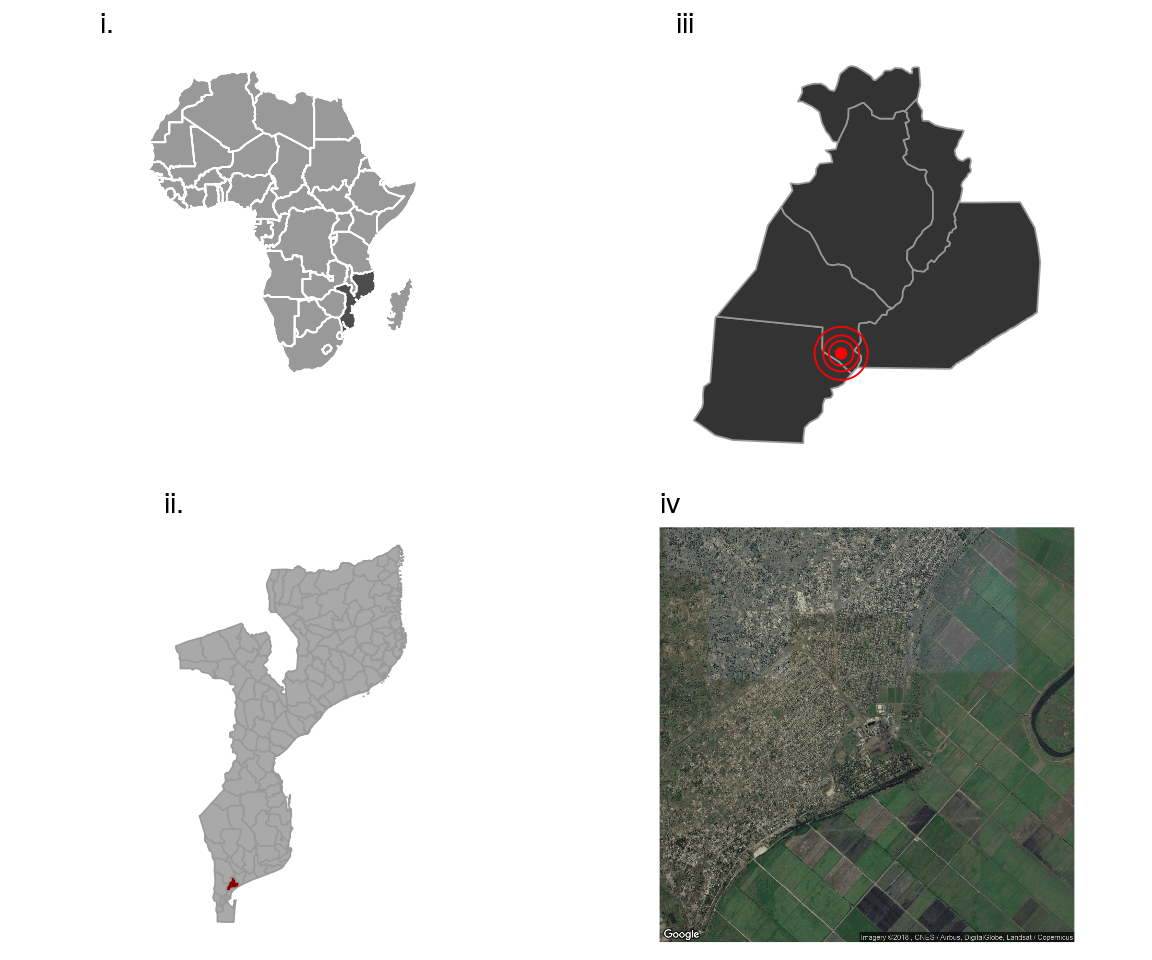
\includegraphics{externalities_files/figure-latex/unnamed-chunk-5-1} \end{center}

We heavily weight towards closer houses to account for the relatively
small travel distances that most mosquitoes fly in normal conditions
(Verdonschot and Besse-Lototskaya 2014).

\subsection{Density}\label{density}

We consider a house's ``herd'' protection level (ie, the protection
conferred to the house through externality) to be the average of the
other houses' non-herd protection levels (ie, 0 if not protected and 1
if protected), weighted by the distance to the house in question. The
below is an illustration of a house (the red x) and the neighboring
houses (circles). The ``weight'' of each house is indicated by the
circle size, and the protection level of the house is indicated by the
shading of the circle.

\begin{center}\includegraphics{externalities_files/figure-latex/unnamed-chunk-6-1} \end{center}

However, this consideration misses one important dimension: density. The
below house's weighted average protection score is identical to that of
the above house. In other words, at the time in question, at both
locations, the percentage of houses with IRS coverage is the same, and
the (weighted) average time since IRS is the same. However, the below
house is likely much more protected than the above, given the
\emph{absolute} number of nearby IRS-protected houses.

\begin{center}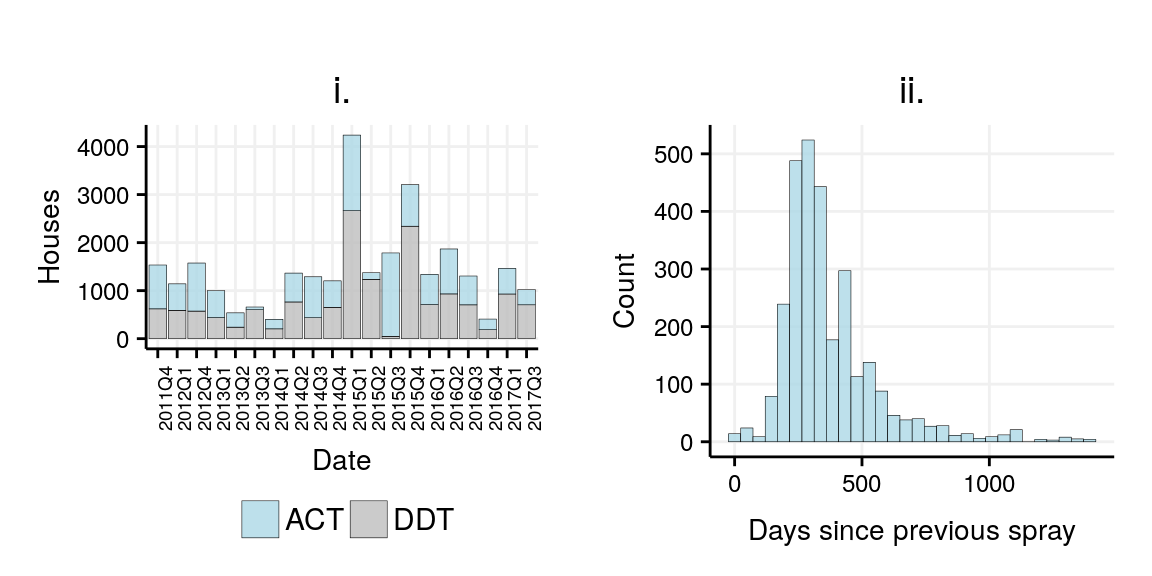
\includegraphics{externalities_files/figure-latex/unnamed-chunk-7-1} \end{center}

In the latter representation, the likelihood of a mosquito landing on a
DDT-affected surface is much higher than the former, even though the
relative IRS coverage for the neighborhood is identical. In order to
account for this, we must take \emph{density} itself into account, ie
the number of houses (and their protection level and proximity) within 1
kilometer.

Our approach is this: rather than using a weighted average of each
household's individual protection score, we instead use a weighted sum.
A particular household's herd protection score at any given time is the
sum of all households' individual protection scores at that time
multiplied by those households' distance weights.

\subsection{Combining them all
together}\label{combining-them-all-together}

The summation of (a) the IRS level of other houses at a certain time,
(b) weighted by the distance of those houses to the house in question,
(c) limited to only the 1 km radius multiplied yields a ``herd
protection score''.

This score is conceptually similar to Cohen and Dupas' quantification of
the positive externalities of ITN (bednet) use in Kenya (Cohen and Dupas
2010) in that it attempts to estimate the protection conferred to
``non-users'' by users and uses a ``weighted sum'' (as opposed to
average). Our approach differs in that the time dimension for IRS is
much more important than ITN (ie, IRS is not a binary but rather a
waning function, as described previously), requiring us to create herd
scores for every day. This is because the protection conferred to a
house by its neighbors may change from one day to the next, when a
neighbor either (a) gets sprayed or (b) leaves ``protected'' status (ie,
due to the end of the 6 months window).

Our approach can be justified in that previous studies have found strong
positive health externalities in malaria interventions related to ITN
coverage (Alaii et al. 2003). No studies exist on positive externalities
for IRS coverage, but to the extent that the mechanisms for the
reduction in infection are similar (reduction in the natural reservoir
of the disease, reduction in the number of vectors, etc.), it is
reasonable to assume similar effects. Additionally, we using weighted
distance for our score calculation (rather than simply defining a radius
threshold) because of previous studies' findings that there is a linear
decline in protection conferred to others with greater distance from an
intervention (Binka et al. 2007)

\subsection{Incorporating into data and
model}\label{incorporating-into-data-and-model}

We calculate a ``herd protection'' score for each location-date
combination (395019 values). Whereas our original model specification
looked like:

\[
\hat{Y_{it}} = \hat{\beta}_{0} +  \hat{\beta}_{1}\text{Season}_{t} * (\hat{\beta}_2{IRS_{it}}*\hat{\beta}_3{IRStime_{it}}) + \alpha_i + \delta_t + \upsilon_{it}
\]

Our new specification incorporates the herd protection value:

\[
\hat{Y_{it}} = \hat{\beta}_{0} +  \hat{\beta}_{1}\text{Season}_{t} * (\hat{\beta}_2{IRS_{it}}*\hat{\beta}_3{IRStime_{it}}) +  \hat{\beta}_4{Herd_{it}} +  \alpha_i + \delta_t + \upsilon_{it}
\]

\(\hat{Y}_{it}\) is the rate of absence. \(\beta_{1}\) is the binary
``season'' variable, imputed from overall district clinical incidence.
Our intervention is whether the residence of the worker in question was
treated in the last year, and, if so, the time since treatment,
represented, respectively, by \(\beta_{2}\) and \(\beta_{3}\).
\(\beta_{4}\) \textbf{represents the distance-weighted herd protection
score}. \(\alpha_i\) represents the time invariant worker fixed effects,
and \(\delta_i\) represents the fixed effect of the particular malaria
season. \(\upsilon\) is the error term.

\newpage

\subsection{Results}\label{results}

\subsubsection{Table}\label{table}

\begin{longtable}[t]{ll}
\caption{\label{tab:unnamed-chunk-8}All absenteeism with herd immunity: model results}\\
\toprule
Term & Estimate\\
\midrule
\endfirsthead
\caption[]{All absenteeism with herd immunity: model results \textit{(continued)}}\\
\toprule
Term & Estimate\\
\midrule
\endhead
\
\endfoot
\bottomrule
\endlastfoot
\addlinespace[1.5em]
\multicolumn{2}{l}{\textbf{Permanent field worker}}\\
\hspace{1em}Malaria season & 2.809 (P<0.001)\\
\hspace{1em}IRS status=After & 1.835 (P<0.001)\\
\hspace{1em}Rainy day & 3.765 (P<0.001)\\
\hspace{1em}Herd protection & -0.003 (P=0.368)\\
\hspace{1em}Malaria season:IRS status=After & -5.106 (P<0.001)\\
\addlinespace[1.5em]
\multicolumn{2}{l}{\textbf{Permanent not field worker}}\\
\hspace{1em}Malaria season & 0.831 (P<0.001)\\
\hspace{1em}IRS status=After & 1.151 (P<0.001)\\
\hspace{1em}Rainy day & 3.835 (P<0.001)\\
\hspace{1em}Herd protection & 0 (P=0.927)\\
\hspace{1em}Malaria season:IRS status=After & -1.66 (P<0.001)\\
\addlinespace[1.5em]
\multicolumn{2}{l}{\textbf{Temporary field worker}}\\
\hspace{1em}Malaria season & -0.188 (P=0.001)\\
\hspace{1em}IRS status=After & -0.254 (P<0.001)\\
\hspace{1em}Rainy day & 0 (P=0.994)\\
\hspace{1em}Herd protection & -0.001 (P=0.006)\\
\hspace{1em}Malaria season:IRS status=After & 0.054 (P=0.568)\\
\addlinespace[1.5em]
\multicolumn{2}{l}{\textbf{Temporary not field worker}}\\
\hspace{1em}Malaria season & 5.772 (P<0.001)\\
\hspace{1em}IRS status=After & -2.187 (P=0.023)\\
\hspace{1em}Rainy day & -1.349 (P=0.003)\\
\hspace{1em}Herd protection & 0.043 (P<0.001)\\
\hspace{1em}Malaria season:IRS status=After & -3.235 (P=0.003)\\*
\end{longtable}

\subsection{Spatial protection
surfaces}\label{spatial-protection-surfaces}

The below shows worker locations and the \emph{average} herd protection
score for the entire study period.

\begin{center}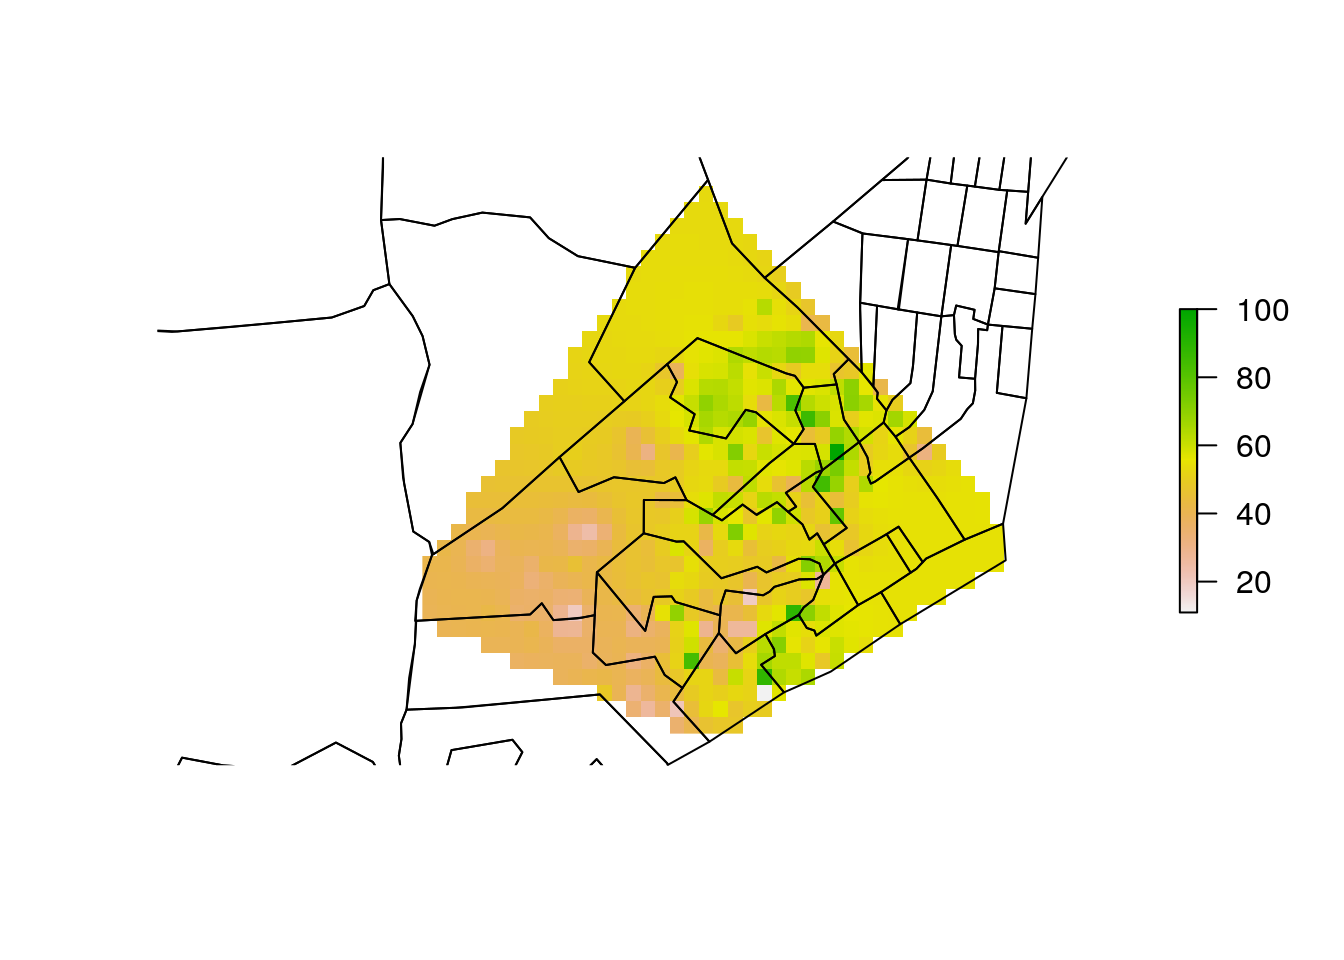
\includegraphics{externalities_files/figure-latex/unnamed-chunk-9-1} \end{center}

The below uses kernel density interpolation to estimate a generalized
protection surface over the entire facility.

\begin{center}\includegraphics{externalities_files/figure-latex/unnamed-chunk-10-1} \end{center}

\begin{center}\includegraphics{externalities_files/figure-latex/unnamed-chunk-11-1} \end{center}

\subsection{Conclusion}\label{conclusion}

Using the approach laid out here, there appears to be a significant
protective effect afforded by the IRS of neighbors. If this approach is
deemed correct, then next steps are determining:

\begin{itemize}
\tightlist
\item
  How to translate the effect into costs and savings (simulation based
  approach at various IRS coverage levels?).
\item
  How / where to report on this in the paper (is this a ``method'' or
  ``result''?).
\end{itemize}

\newpage

\subsection{Appendix}\label{appendix}

\subsubsection{Theoretical protection
surface}\label{theoretical-protection-surface}

The below shows a theoretical protection surface assuming (a) uniform
distribution of residences, (b) random distribution of IRS over time,
but never going beyond 6 months between sprays.

\paragraph{100 workers}\label{workers}

\begin{center}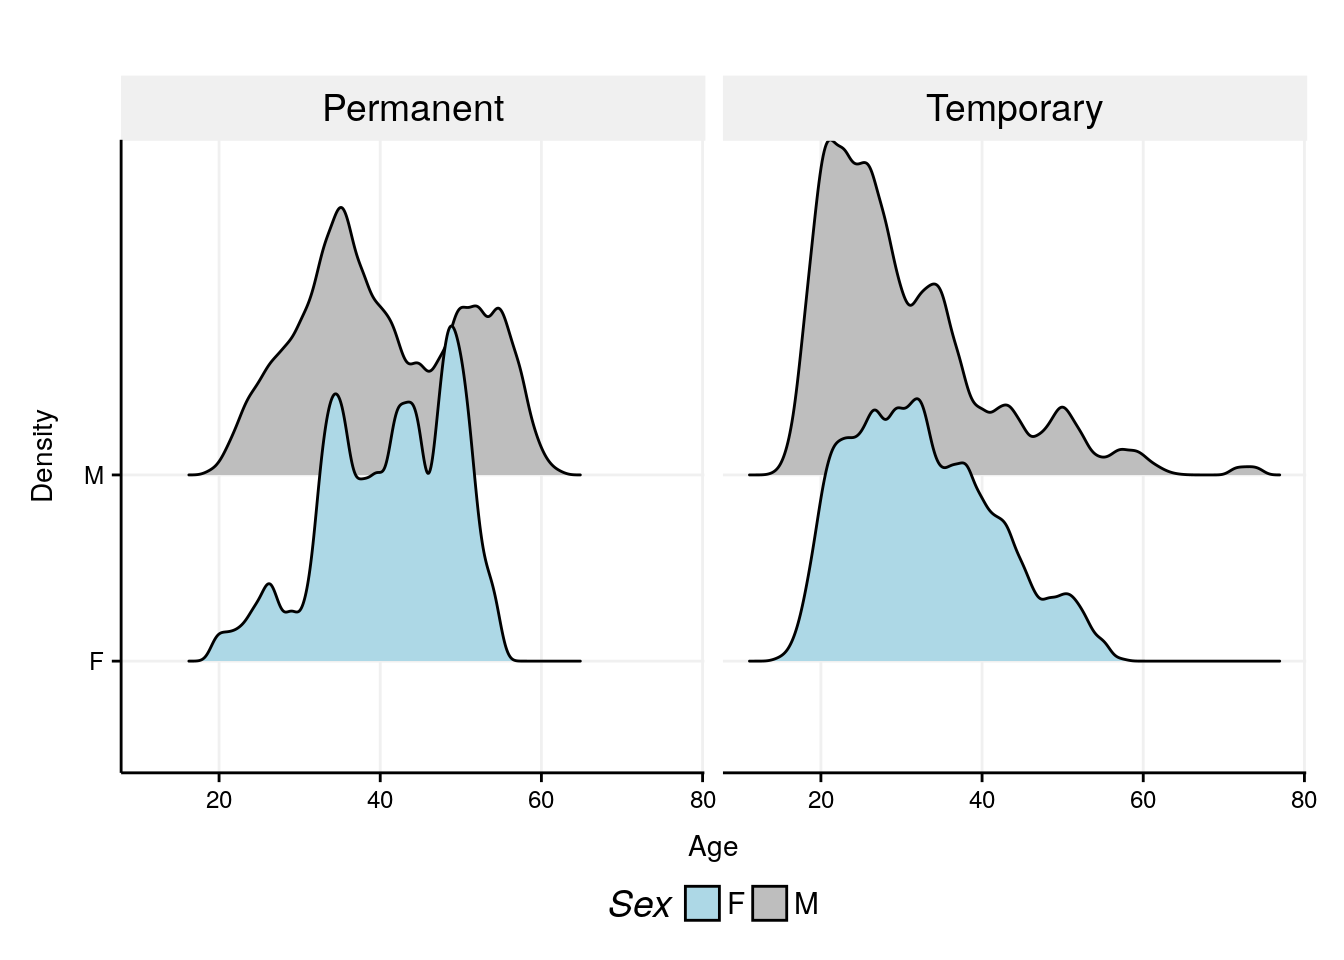
\includegraphics{externalities_files/figure-latex/unnamed-chunk-13-1} \end{center}

\paragraph{1000 workers}\label{workers-1}

\begin{center}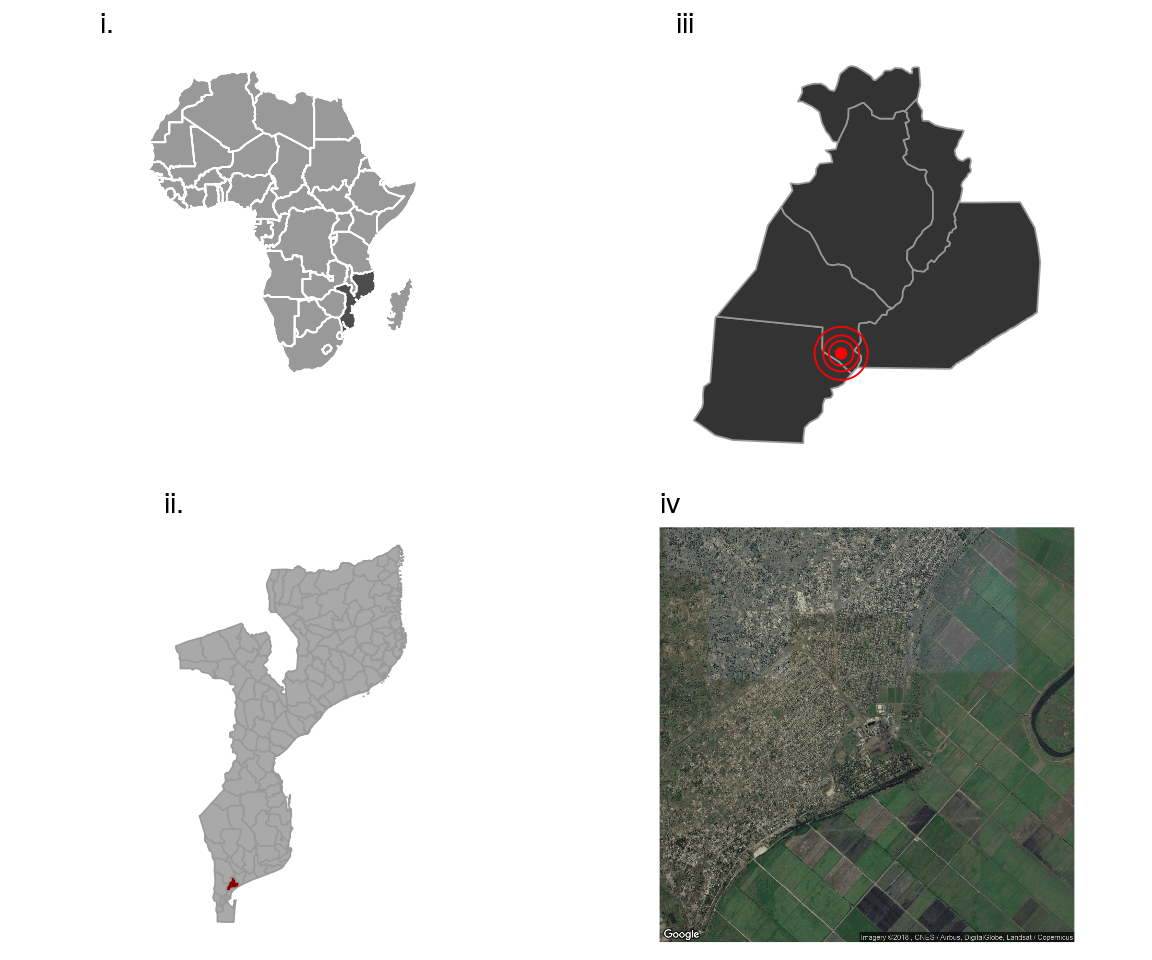
\includegraphics{externalities_files/figure-latex/unnamed-chunk-14-1} \end{center}

\paragraph{3000 workers}\label{workers-2}

\begin{center}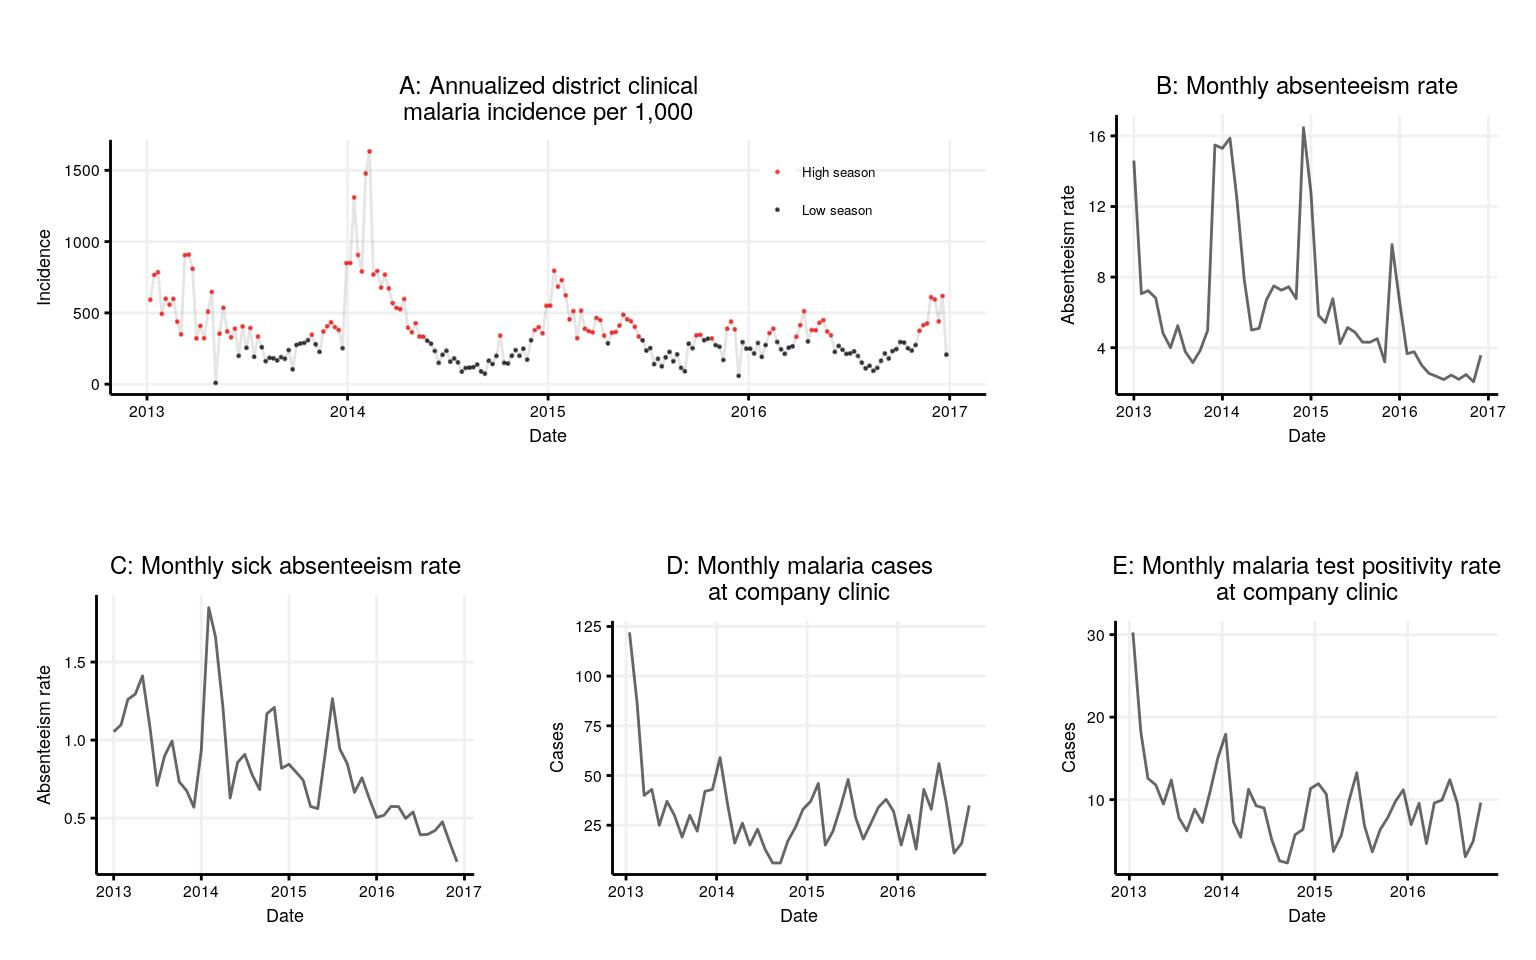
\includegraphics{externalities_files/figure-latex/unnamed-chunk-15-1} \end{center}

\section*{References}\label{references}
\addcontentsline{toc}{section}{References}

\hypertarget{refs}{}
\hypertarget{ref-Alaii2003FactorsAU}{}
Alaii, Jane A., William A. Hawley, Margarette S. Kolczak, Feiko O Ter
Kuile, John E. Gimnig, John Vulule, Amos Odhacha, Aggrey J Oloo, Bernard
L. Nahlen, and Penelope A Phillips-Howard. 2003. ``Factors Affecting Use
of Permethrin-Treated Bed Nets During a Randomized Controlled Trial in
Western Kenya.'' \emph{The American Journal of Tropical Medicine and
Hygiene} 68 4 Suppl: 137--41.

\hypertarget{ref-Binka2007}{}
Binka, F. N., A. Kubaje, M. Adjuik, L. A. Williams, C. Lengeler, G. H.
Maude, G. E. Armah, B. Kajihara, J. H. Adiamah, and P. G. Smith. 2007.
``Impact of Permethrin Impregnated Bednets on Child Mortality in
Kassena-Nankana District, Ghana: A Randomized Controlled Trial.''
\emph{Tropical Medicine \& International Health} 1 (2). Wiley-Blackwell:
147--54.
doi:\href{https://doi.org/10.1111/j.1365-3156.1996.tb00020.x}{10.1111/j.1365-3156.1996.tb00020.x}.

\hypertarget{ref-Bukirwa2009}{}
Bukirwa, H., V. Yau, R. Kigozi, S. Filler, L. Quick, M. Lugemwa, G.
Dissanayake, M. Kamya, F. Wabwire-Mangen, and G. Dorsey. 2009.
``Assessing the Impact of Indoor Residual Spraying on Malaria Morbidity
Using a Sentinel Site Surveillance System in Western Uganda.''
\emph{American Journal of Tropical Medicine and Hygiene} 81 (4).
American Society of Tropical Medicine; Hygiene: 611--14.
doi:\href{https://doi.org/10.4269/ajtmh.2009.09-0126}{10.4269/ajtmh.2009.09-0126}.

\hypertarget{ref-Cohen2010}{}
Cohen, Jessica, and Pascaline Dupas. 2010. ``Free Distribution or
Cost-Sharing? Evidence from a Randomized Malaria Prevention
Experiment.'' \emph{Quarterly Journal of Economics} 125 (1). Oxford
University Press (OUP): 1--45.
doi:\href{https://doi.org/10.1162/qjec.2010.125.1.1}{10.1162/qjec.2010.125.1.1}.

\hypertarget{ref-Tukei2017}{}
Tukei, Betty Bawuba, Andy Beke, and Héctor Lamadrid-Figueroa. 2017.
``Assessing the Effect of Indoor Residual Spraying (IRS) on Malaria
Morbidity in Northern Uganda: A Before and After Study.'' \emph{Malaria
Journal} 16 (1). Springer Nature.
doi:\href{https://doi.org/10.1186/s12936-016-1652-4}{10.1186/s12936-016-1652-4}.

\hypertarget{ref-Verdonschot2014}{}
Verdonschot, Piet F.M., and Anna A. Besse-Lototskaya. 2014. ``Flight
Distance of Mosquitoes (Culicidae): A Metadata Analysis to Support the
Management of Barrier Zones Around Rewetted and Newly Constructed
Wetlands.'' \emph{Limnologica - Ecology and Management of Inland Waters}
45 (March). Elsevier BV: 69--79.
doi:\href{https://doi.org/10.1016/j.limno.2013.11.002}{10.1016/j.limno.2013.11.002}.

\hypertarget{ref-White2011}{}
White, Michael T, Jamie T Griffin, Thomas S Churcher, Neil M Ferguson,
María-Gloria Basáñez, and Azra C Ghani. 2011. ``Modelling the Impact of
Vector Control Interventions on Anopheles Gambiae Population Dynamics.''
\emph{Parasites \& Vectors} 4 (1). Springer Nature: 153.
doi:\href{https://doi.org/10.1186/1756-3305-4-153}{10.1186/1756-3305-4-153}.


\end{document}
